\chapter{SUSY searches in Hadronic Final States}
\label{chap:SUSYsearches}

In this chapter a model independent search for \ac{SUSY} in hadronic final states with $\met$ using the $\alphat$ variable and b-quark multiplicity is introduced and described in detail. The results presented are based on a data sample of pp collisions collected in 2012 at $\com =$8 \TeV, corresponding to an integrate luminosity of 11.7$\pm$0.5 fb$^{-1}$.

The kinematic variable $\alphat$ is motivated as a variable to provide strong rejections of QCD backgrounds, whilst maintaining sensitivity to possible a \ac{SUSY} signal within Section (\ref{sec:alphatintroduction}). The search and trigger strategy in addition to the event reconstruction and selection are outlined within Sections (\ref{subsec:searchstrategy}-\ref{subsec:eventselection}). 

The method in which the \ac{SM} background is estimated using an analytical technique to improve statistical precision at higher b-tag multiplicities is detailed within Section (\ref{subsec:backgroundestimation}), with a discussion on the impact of b-tagging and mis-tagging scale factors between data and MC on any background predictions. Finally a description of the formulation of appropriate systematic uncertainties applied to the background predictions to account for theoretical uncertainties and limitations in the simulation modelling of event kinematics and instrumental effects is covered in Section (\ref{subsec:sysuncertainties}).


In addition to the $\alphat$ search, a complimentary technique is discussed as a means to predict the distribution of 3 and 4 reconstructed b-quark jets in an event in Section (\ref{sec:templatemethod}). The recent discovery of the Higgs boson has made third-generation ``Natural \ac{SUSY}'' models attractive, given that light top and bottom squarks are a candidate to stabilise divergent loop corrections to the Higgs boson mass.

Using the $\alphat$ search as a base, a simple templated fit is employed to estimate the \ac{SM} background in higher b-tag multiplicities (3-4) from a region of a low number of reconstructed b-jets (0-2). The predictions using this technique are first tested in simulation before being compared to the \ac{SM} background predictions obtained from the $\alphat$ search.  

The experimental reach of the analysis discussed within this thesis is interpreted in two classes of \ac{SMS} models, the topologies of which are detailed in Section (\ref{subsec:sms}). The \ac{SMS} models considered in this analysis are summaries in Table \ref{tab:sms_model_table}. For each model, the \ac{LSP} is assumed to be the lightest neutralino. 

Within Table \ref{tab:sms_model_table} is also defined reference points, parameterised in terms of parent gluino/squark and \ac{LSP} sparticle masses, m$_{parent}$ and m$_{LSP}$, respectively, which are used within the following two chapters to demonstrate potential yields within the signal region of the search. The masses are chosen to reflect parameter space which is within the expect sensitivity reach of the search.

\begin{table}[h!]
\begin{center}
\begin{tabular*}{0.75\textwidth}{@{\extracolsep{\fill}}llcc}
\cline{1-4}
Model & Production/decay mode &  \multicolumn{2}{c}{Reference model}\\ 
&& m$_{parent}$ & m$_{LSP}$ \\  \cline{1-4}
G1 (T1) & $ pp \rightarrow \widetilde{g}\widetilde{g}^{*} \rightarrow q\bar{q}\widetilde{\chi}^{0}_{1}q\bar{q}\widetilde{\chi}^{0}_{1}$ & 700 & 300 \\
G2 (T1bb) & $ pp \rightarrow \widetilde{g}\widetilde{g}^{*} \rightarrow b\bar{b}\widetilde{\chi}^{0}_{1}b\bar{b}\widetilde{\chi}^{0}_{1}$ & 900 & 500 \\
G3 (T1tt) & $ pp \rightarrow \widetilde{g}\widetilde{g}^{*} \rightarrow t\bar{t}\widetilde{\chi}^{0}_{1}t\bar{t}\widetilde{\chi}^{0}_{1}$ & 850 & 250 \\
D1 (T2) & $ pp \rightarrow \widetilde{q}\widetilde{q}^{*} \rightarrow q\widetilde{\chi}^{0}_{1}\bar{q}\widetilde{\chi}^{0}_{1}$ & 600 & 250 \\
D2 (T2bb) & $ pp \rightarrow \widetilde{b}\widetilde{b}^{*} \rightarrow b\widetilde{\chi}^{0}_{1}\bar{b}\widetilde{\chi}^{0}_{1}$ & 500 & 150 \\
D3 (T2tt) & $ pp \rightarrow \widetilde{t}\widetilde{t}^{*} \rightarrow t\widetilde{\chi}^{0}_{1}\bar{t}\widetilde{\chi}^{0}_{1}$ & 400 & 0 \\
\cline{1-4}
\end{tabular*}
\end{center}
\caption[A summary of the \ac{SMS} models interpreted in this analysis, involving both direct (D) and glunio-induced (G) production of squarks and their decays.]{A summary of the \ac{SMS} models interpreted in this analysis, involving both direct (D) and glunio-induced (G) production of squarks and their decays. Reference models are also defined in terms of parent and \ac{LSP} sparticle mass }
\label{tab:sms_model_table}
\end{table}

\section{An introduction to the \alphat search}
\label{sec:alphatintroduction}

The experimental signature of \ac{SUSY} signal in the hadronic channel would manifest as a final state containing energetic jets and $\met$. The search focuses on topologies where new heavy supersymmetric, R-parity conserving particles are pair-produced in pp collisions. These particles decaying to a \ac{LSP} escape the detector undetected, leading to significant missing energy and missing hadronic transverse energy,

\begin{equation}
\mht =  \lvert \sum_{i=1}^{n} p_{T}^{jet_{i}} \rvert,
\end{equation}

defined as the vector sum of the transverse energies of jets selected in an event. Energetic jets produced in the decay of these supersymmetric particles also 
can produce significant visible transverse energy, 

\begin{equation}
\theht = \sum_{i=1}^{n} E_{T}^{jet_{i}},
\end{equation}

defined as the scalar sum of the transverse energies of jets selected in an event.

A search within this channel is greatly complicated in a hadron collider environment, where the overwhelming background comes from inherently balanced multi-jet (``QCD'') events which are produced with an extremely large cross section as demonstrated within Figure \ref{fig:htqcdbackground}. $\met$ can appear in such events with a substantial mis-measurement of jet energy or missed objects due to detector miscalibration or noise effects. 

\begin{figure}[!h]

\centering
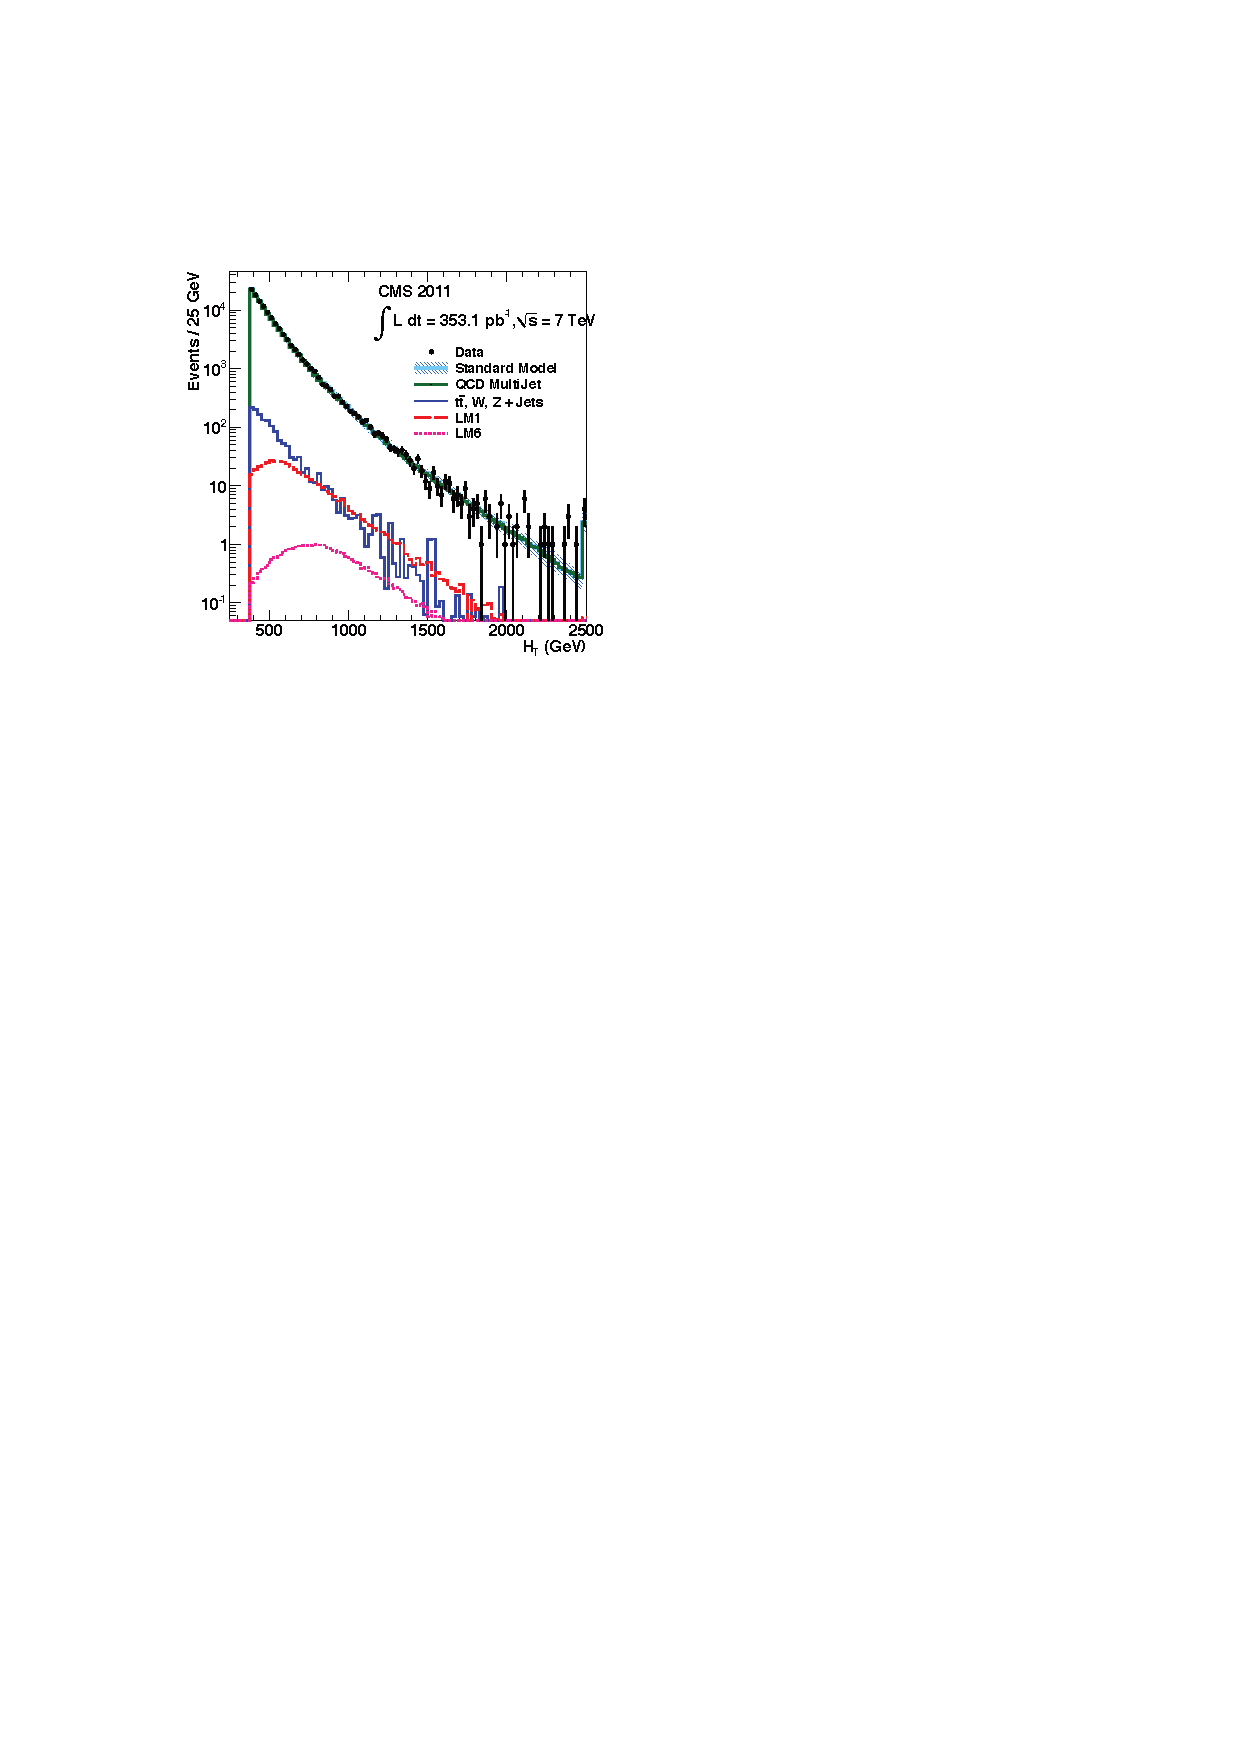
\includegraphics[width=0.60\textwidth]{plots/nocuts_htdistribution.pdf}
\caption[Reconstructed offline \theht for 11.7fb$^{-1}$ of data after a basic pre-selection.]{Reconstructed offline $\theht$ for 11.7fb$^{-1}$ of data after a basic pre-selection. Sample is collected from prescaled \theht triggers. Overlaid are expectations from MC simulation of \ac{EWK} processes as well as a reference signal model (labelled D2 from Table.\ref{tab:sms_model_table}).}  
\label{fig:htqcdbackground}
\end{figure}

Additional \ac{SM} background from \ac{EWK} processes with genuine $\met$ from escaping neutrinos comprise the irreducible background within this search and come mainly from:

\begin{itemize}
\item $Z \rightarrow \nu\bar{\nu} +$ jets,
\item $W \rightarrow l\nu$ + jets in which a lepton falls outside of detector acceptance, or the lepton decays hadronically $\tau \rightarrow$ had ,
\item $t\bar{t}$ with at least one leptonic W decay,
\item small background contributions from DY, single top and Diboson (WW,ZZ,WZ) processes.
\end{itemize}

The search is designed to have a strong separation between events with genuine and ``fake'' $\met$ which is achieved primarily though the dimensionless kinematic variable, $\alphat$ \cite{PhysRevLett.101.221803}\cite{CMS:2008vya}.

\subsection{The $\alphat$ variable}
\label{subsec:alphatvariable}

For a perfectly measured di-jet QCD event, conservation laws dictate that they must be produced back-to-back and of equal magnitude. However in di-jet events with real $\met$, both of these jets are produced independently of one another, depicted in Figure \ref{fig:susytopology}.
\begin{figure}[!h]
\centering
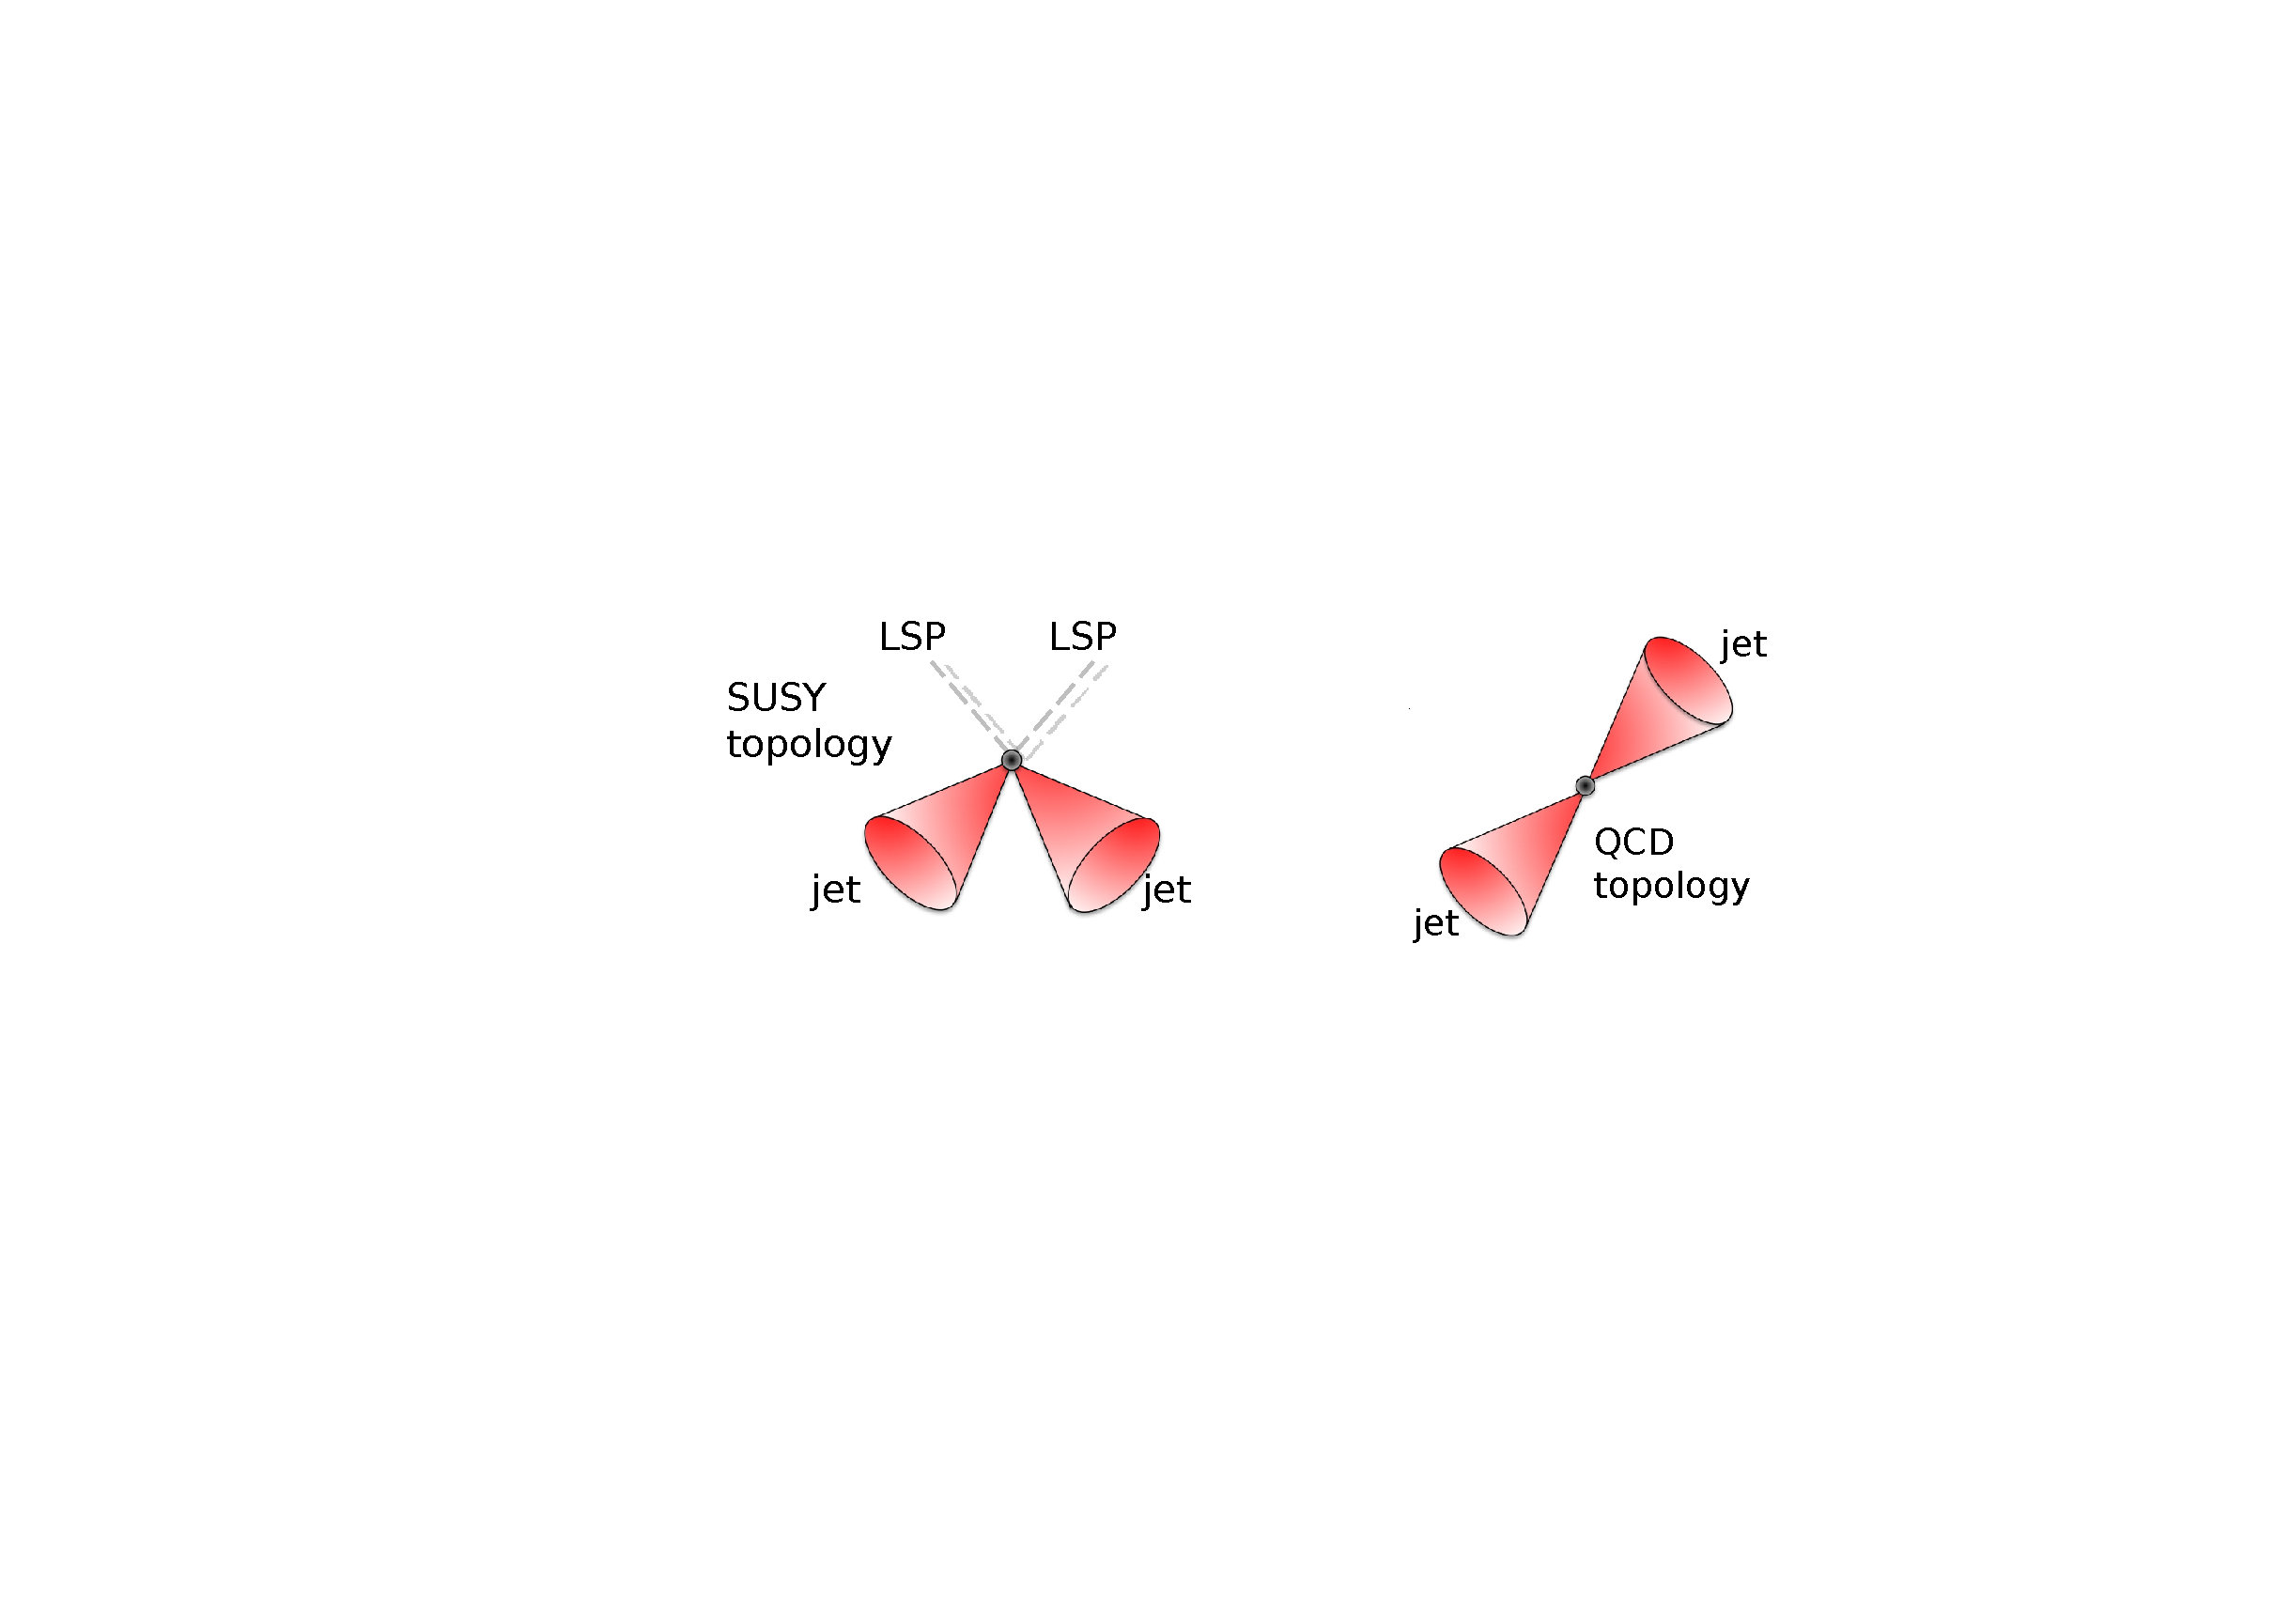
\includegraphics[width=0.90\textwidth]{plots/susy_topology.pdf}
\caption[The event topologies of background QCD diet events (right) and a generic \ac{SUSY} signature with genuine $\met$ (left).]{The event topologies of background QCD diet events (right) and a generic \ac{SUSY} signature with genuine $\met$ (left).}  
\label{fig:susytopology}
\end{figure}

 Exploiting this feature leads to the formulation of $\alphat$ in di-jet systems defined as,

\begin{equation}
\alphat = \frac {E^{j2}_{T}}{M_{T}},
\end{equation} 

where $E^{j2}_{T}$ is the transverse energy of the least energetic of the two jets and $M_{T}$ defined as:

\begin{equation}
\label{eq:transmass}
M_{T} = \sqrt{\left(\sum^{2}_{i=1}E^{j_{i}}_{T}\right)^{2}-\left(\sum^{2}_{i=1}p^{j_{i}}_{x}\right)^{2}-\left(\sum^{2}_{i=1}p^{j_{i}}_{y}\right)^{2}} \equiv \sqrt{H_{T}^{2} - \mht^{2}} .
\end{equation}

A perfectly balanced di-jet event i.e. $E_{T}^{j_{1}} = E_{T}^{j_{2}}$ would give an $\alphat = 0.5$, where as events with jets which are not back-to-back, for example in events in which
a W or Z recoils off a system of jets, $\alphat$ can achieve values in excess of 0.5.

$\alphat$ can be extended to apply to any arbitrary number of jets, undertaken by modelling a system of $n$ jets as a di-jet system, through the formation of two pseudo-jets \cite{CMS-PAS-SUS-09-001}. The two pseudo-jets are built by merging the jets present in the event such that the 2 pseudo-jets are chosen to be as balanced as possible, i.e the $\Delta$ \theht $\equiv \lvert E_{T}^{pj_{1}} - E_{T}^{pj_{2}}\rvert$ is minimised between the two pseudo jets. Using Equation (\ref{eq:transmass}), $\alphat$ can be rewritten as,

\begin{equation}
\alphat = \frac{1}{2} \frac {\theht - \Delta\theht}{\sqrt{\theht^{2}-\mht^{2}}}= \frac{1}{2}\frac{1-\Delta\theht/\theht}{\sqrt{1-(\mht/\theht)^{2}}}.
\end{equation}

The distribution of $\alphat$ for the two jet categories used within this analysis, 2,3 and $\geq 4$ jets, is shown in the Figure.\ref{fig:fullalphatdistribution}, demonstrating the ability of the $\alphat$ variable to discriminate between multi jet events and \ac{EWK} processes with genuine $\met$ in the final state.  

\begin{figure}[ht]
\centering
\begin{minipage}[b]{0.48 \linewidth}
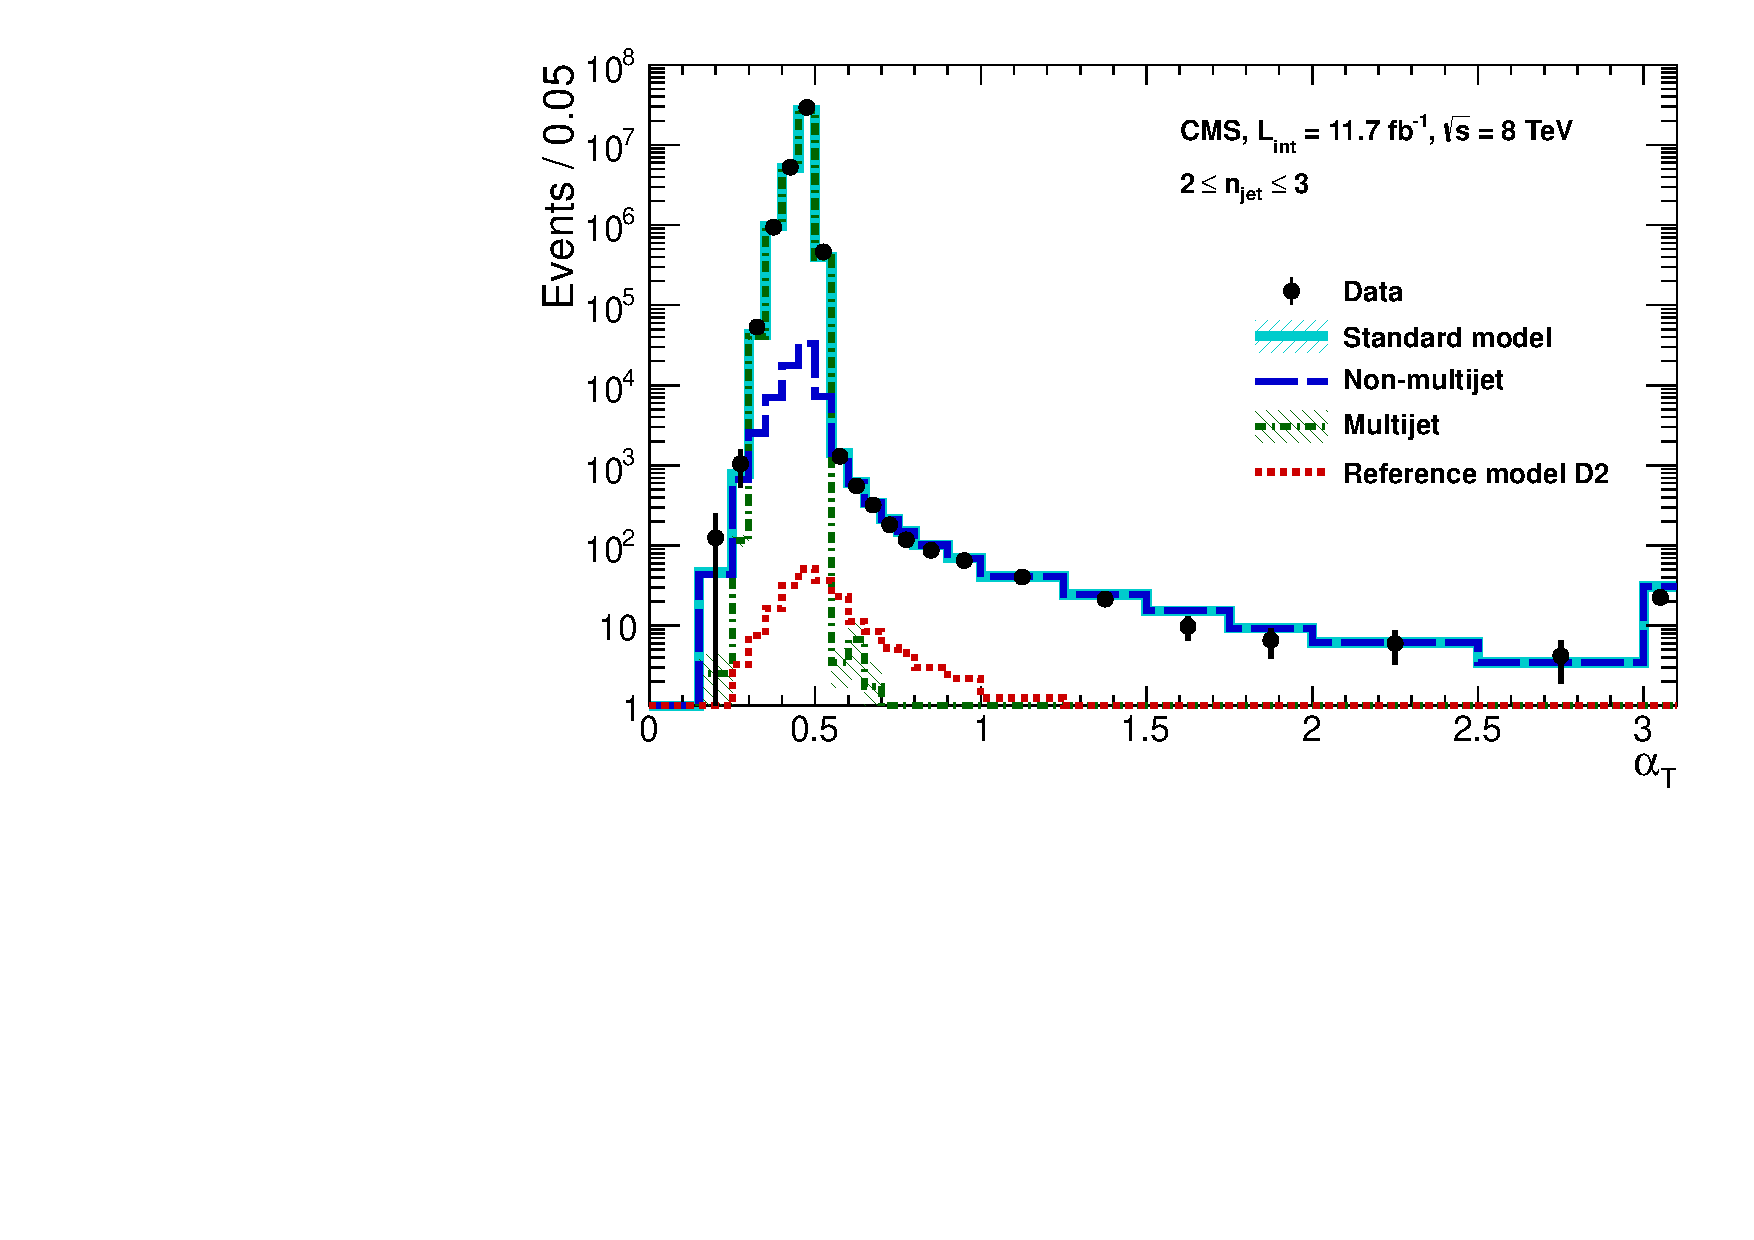
\includegraphics[width = 1.0\linewidth,height = 7.0cm]{plots/alphat_low.pdf}
\end{minipage}
\quad
\begin{minipage}[b]{0.48\linewidth}
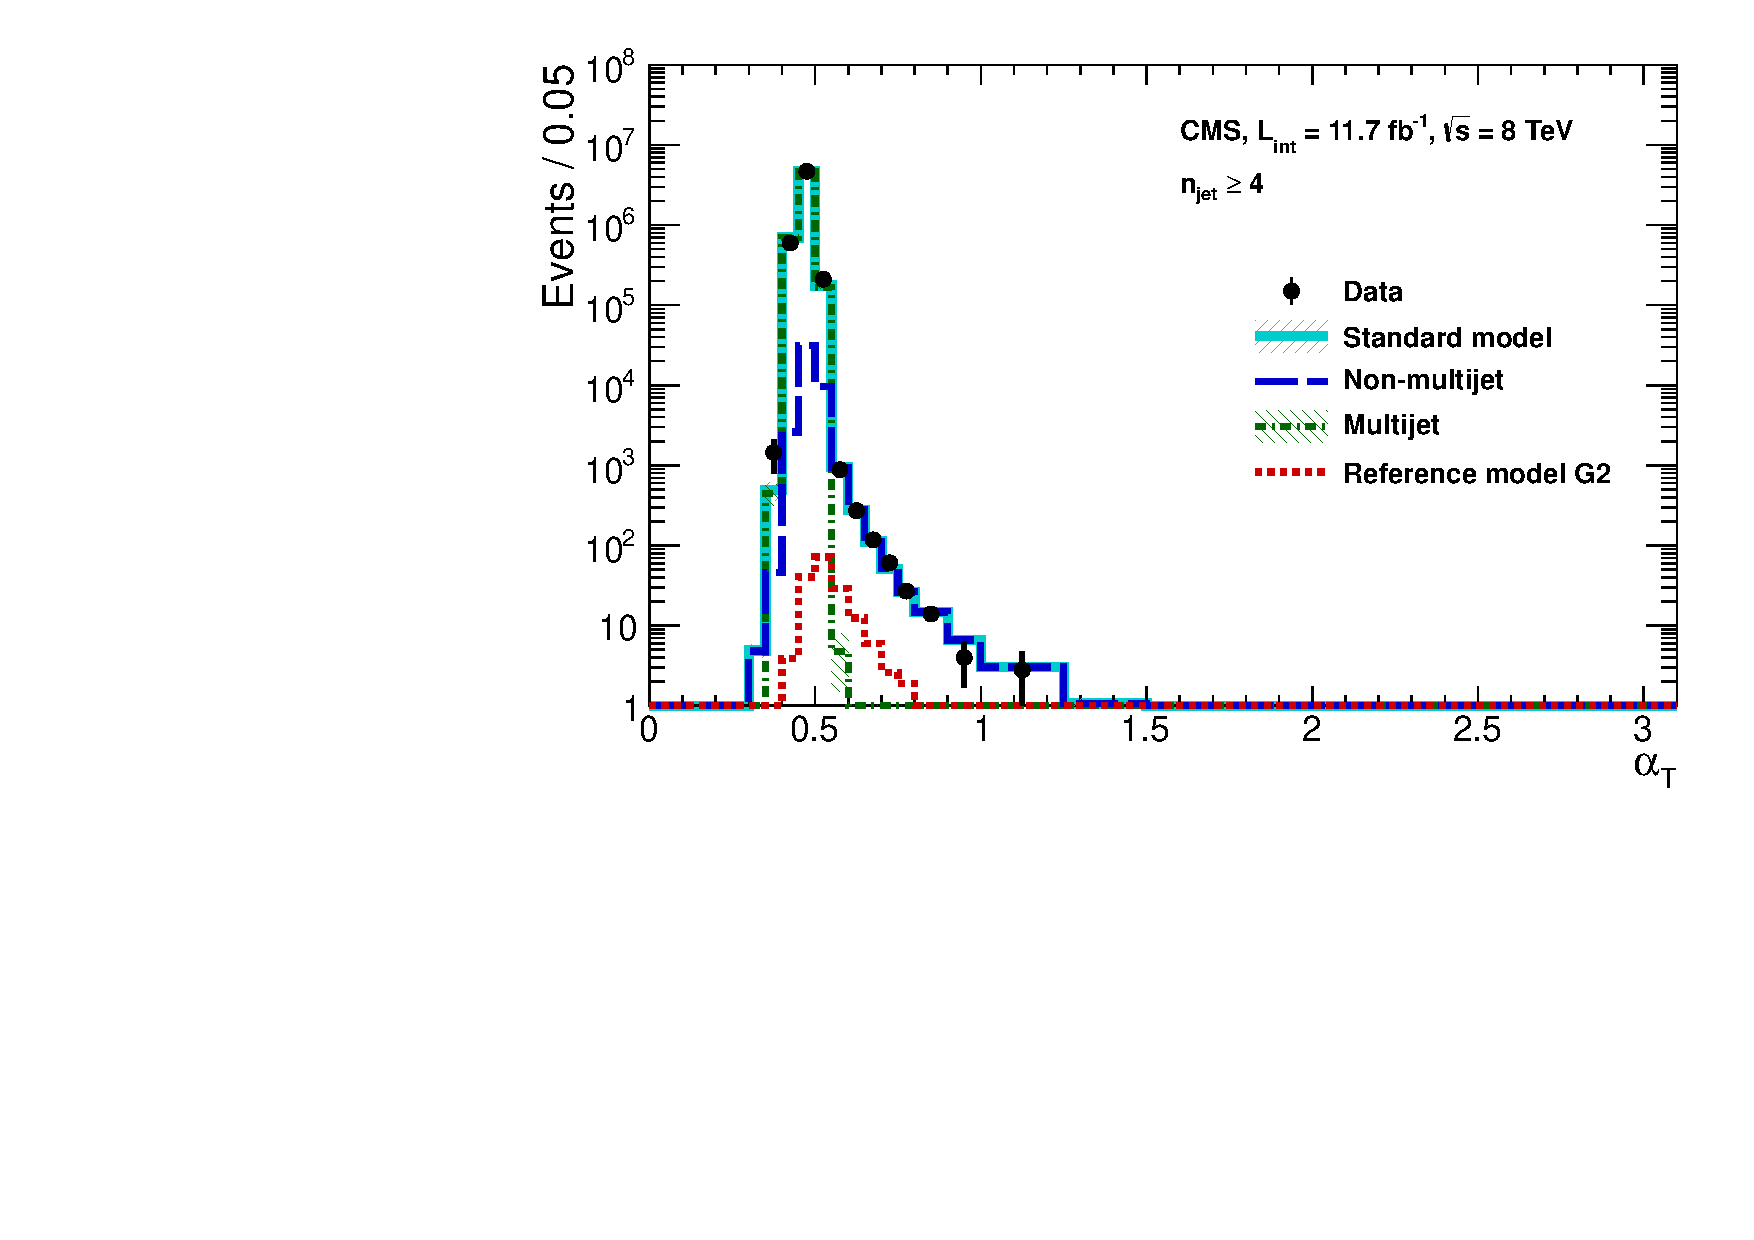
\includegraphics[width = 1.0\linewidth, height = 7.0cm]{plots/alphat_high.pdf}
\end{minipage}
\caption[ The $\alphat$ distributions for the low 2-3 (left) and high $\geq 4$ (right) jet multiplicities after a full analysis selection and shown for $\theht > 375$.]{The $\alphat$ distributions for the low 2-3 (left) and high $\geq 4$ (right) jet multiplicities after a full analysis selection and shown for $\theht > 375$ . Data is collected using both prescaled $\theht$ triggers and dedicated $\alphat$ triggers for below and above $\alphat = 0.55$ respectively. . Expected yields as given by simulation are also shown for multijet events (green dash-dotted line), \ac{EWK} backgrounds with genuine $\met$ (blue long-dashed line), the sum of all \ac{SM} processes (cyan solid line) and the reference signal model D2 (left, red dotted line) or G2 (right, red dotted line). }
\label{fig:fullalphatdistribution}
\end{figure}

The $\alphat$ requirement used within the search is chosen to be $\alphat >$ 0.55 to ensure that the QCD multijet background is negligible even in the presence of moderate jet mis-measurement. There still remains other effects which can cause multijet events to artificially have a large $\alphat$ value, which are discussed in detail in Section (\ref{subsec:eventselection}).  


\section{Search Strategy}
\label{subsec:searchstrategy}

The aim of the analysis presented in this thesis is to identify an excess of events in data over the \ac{SM} background expectation in multi-jet final states and significant $\met$. The essential suppression of the dominant QCD background for such a search is addressed by the $\alphat$ variable described in the previous section. For estimation of the remaining \ac{EWK} backgrounds, three independent data control samples are used to predict the different processes that compose the background :

\begin{itemize}
\item \mupjets to determine W + jets, \ttbar and single top backgrounds,
\item \gpjets  to determine the irreducible \zinv + jets background,
\item \dimupjets to determine the irreducible \zinv + jets background.
\end{itemize}

These control samples are chosen to both be rich in specific \ac{EWK} processes, be free of QCD multi-jet events and to also be kinematically similar to the hadronic signal region that they are estimating the backgrounds of, see Section (\ref{subsec:controlsampledefinition}).

To remain inclusive to a large range of possible \ac{SUSY} models, the signal region is binned in the following categories to allow for increased sensitivity in the interpretation of results for different \ac{SUSY} topologies:

\begin{itemize}

\item[] \textbf{Sensitivity to a range of \ac{SUSY} mass splittings}

The hadronic signal region is defined by \theht $>$ 275, divided into eight bins in \theht. 

\begin{itemize}
\item Two bins of width 50 \GeV in the range 275 $<$ \theht $<$ 375 \GeV,
\item five bins of width 100 \GeV in the range 375 $<$ \theht$<$ 875 \GeV,
\item and a final open bin, \theht $>$ 875 \GeV.
\end{itemize}

The choice at low \theht is driven primarily by trigger constraints. The mass difference between the \ac{LSP} and the particle that it decays from is an important factor in the amount of hadronic activity in the event. 

A large mass splitting will lead to hard high \pt jets which contribute to the \theht sum. From Figure \ref{fig:htqcdbackground} it can be seen that the \ac{SM} background falls sharply at high \theht values, therefore a large number of \theht bins will lead to easier of identification of such signals. Conversely smaller mass splittings lead to softer jet \pt's which will subsequently fall into the lower \theht range.

\item[] \textbf{Sensitivity to production method of \ac{SUSY} particles}

The production mechanism of any potential \ac{SUSY} signal can lead to different event topologies. One such way to discriminate between gluino ($g\widetilde{g}$ - ``high multiplicity''), and direct squark ($q\widetilde{q}$ - ``low multiplicity'') induced production of \ac{SUSY} particles is realised through the number of reconstructed jets in the final state.  

The analysis is thus split into two jet categories : 2-3 jets , $\geq$ 4 jets to give sensitivity to both of these mechanisms. 

\item[] \textbf{Sensitivity to  ``Natural \ac{SUSY}'' via tagging jets from b-quarks}

Jets originating from bottom quarks (b-jets) are identified through vertices that are displaced with respect to the primary interaction. The algorithm used to tag b-jets is the \acf{CSVM} tagger, described within Section (\ref{subsec:cmsobjects-btagging}). A cut is placed on the discriminator variable of $> 0.679$, leading to a gluon/light-quark mis-tag rate of 1\% and a jet p$_{\text{T}}$ dependant b-tagging efficiency of 60-70\% \cite{btag8tev}.

Natural \ac{SUSY} models would be characterised through final-state signatures rich in bottom quarks. A search relying on methods to identify jets originating from bottom quarks through b-tagging, will significantly improve the sensitivity to this class of signature. 

This is achieved via the binning of events in the signal region according to the number of b-tagged jets reconstructed in each event, in the following: 0,1,2,3,$\geq$ 4 b-tag categories . In the highest $\geq$ 4 b-tag category due to a limited number of expected signal and background, just three \theht bins are employed: 275-325 \GeV, 325-375 \GeV, $\geq$ 375 \GeV.

This characterisation is identically mirrored in all control samples, with the information from all samples and b-tag categories used simultaneously in the likelihood model (see Chapter \ref{chap:SUSYresults}) in order to interpret the results in a coherent and powerful way.

\end{itemize}
 
 The combination of the \theht, jet multiplicity and b-tag categorisation of the signal region as described above, resultantly leads to 67 different bins in which the analysis is interpreted in, which is depicted in Figure \ref{fig:analysisbinning}. 
 
 \begin{figure}[!h]
 \centering
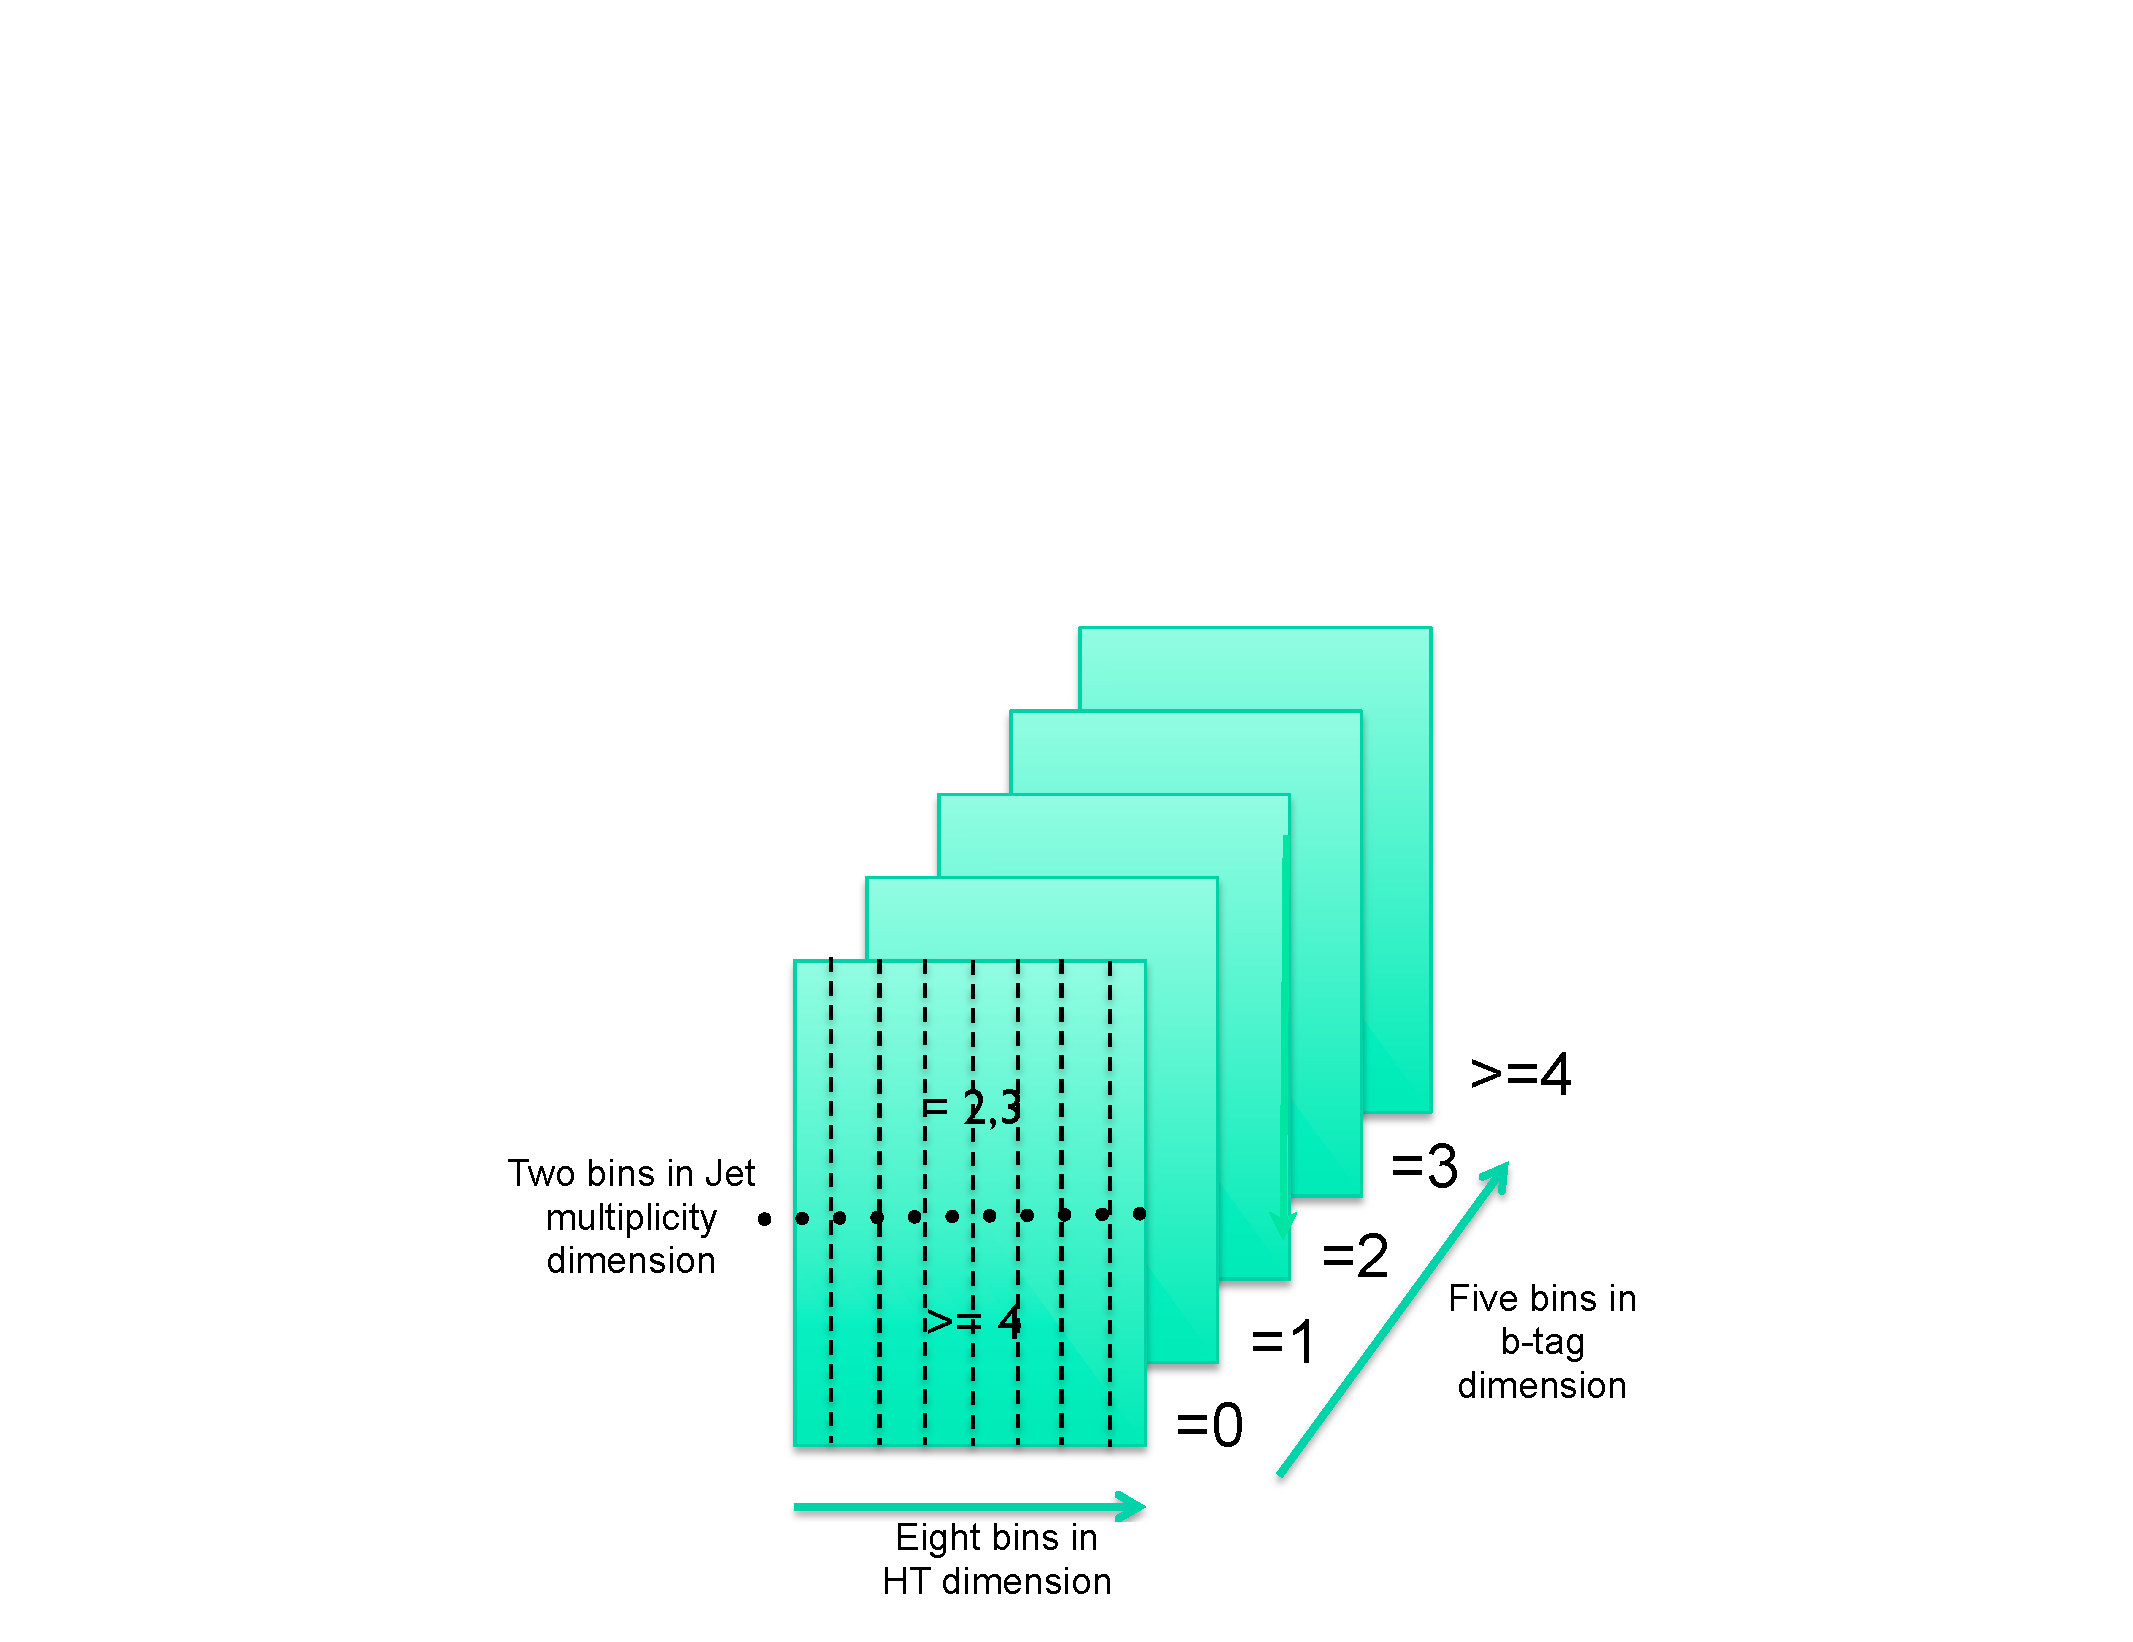
\includegraphics[width=0.70\textwidth]{plots/analysis_binning.pdf}
\caption[Pictorial depiction of the analysis strategy employed by the $\alphat$ search to increase sensitivity to a wide spectra of \ac{SUSY} models.]{Pictorial depiction of the analysis strategy employed by the $\alphat$ search to increase sensitivity to a wide spectra of \ac{SUSY} models.}  
\label{fig:analysisbinning}
\end{figure}



\subsection{Physics Objects}
\label{subsec:physicsobjects}

The physics objects used in the analysis defined below, follow the recommendation of the various \ac{CMS} \acf{POGs}. 

\begin{itemize}

\item \textbf{Jets}

The jets used in this analysis are CaloJets, reconstructed as described in Section (\ref{subsec:cmsobjects-jets}) using the anti-k$_{T}$ jet clustering algorithm. 

To ensure the jet object falls within the calorimeter systems a pseudo-rapidity requirement of \abeta $<$ 3 is applied. Each jet must pass a ``loose'' identification criteria to reject jets resulting from unphysical energy, the criteria of which are detailed in Table \ref{tab:jetidtable} \cite{CMS-PAS-JME-09-008}.

\begin{table}[h!]
\begin{center}
\begin{tabulary}{0.8\textwidth}{LL}
\cline{1-2}
Variable & Definition \\ 
\cline{1-2}
f$_{HPD} < 0.98$ \qquad\qquad\qquad\qquad\qquad\qquad & Fraction of jet energy contributed from ``hottest'' \ac{HPD}, which rejects \ac{HCAL} noise.  \\
f$_{EM} > 0.01$ & Noise from the \ac{HCAL} is further suppressed by requiring a minimal electromagnetic component to the jet f$_{EM}$. \\
 N$^{90}_{hits} \geq$ 2 & Jets that have $>$ 90\% of its energy from a single chanel are rejected, to serve as a safety net that catches jets arising from undiagnosed noisy channels.\\

\cline{1-2}
\end{tabulary}
\end{center}
\caption[Jet Identification criteria for the ``loose" CaloJet ID used with the analysis.]{Jet Identification criteria for the ``loose" CaloJet ID, used to reject reconstructed jets resulting from fake calorimeter deposits representing unphysical energy.}
\label{tab:jetidtable}
\end{table}

\item \textbf{Muons}

Muons are selected in the \mupjets and \dimupjets control samples, and vetoed in the signal region. The same cut based identification criteria is applied to muons in both search regions and is summarised in Table \ref{tab:muonidtable} \cite{1748-0221-7-10-P10002}.

\begin{table}[h!]
\begin{center}
\begin{tabular*}{0.5\textwidth}{@{\extracolsep{\fill}}ll}
\cline{1-2}
Categories & Criteria \\ 
\cline{1-2}
Global Muon & True \\
PFMuon & True \\
$\chi^{2}$ & $<$ 10 \\
Muon chamber hits & $>$ 0 \\
Muon station hits & $>$ 1 \\
Transvere impact d$_{xy}$ & $<$ 0.2mm \\
Longitudinal distance d$_{z}$ & $<$ 0.5mm \\
Pixel hits & $>$ 0\\
Track layer hits & $>$ 5 \\
PF Isolation (DeltaB corrected) & $<$0.12 \\
\cline{1-2}
\end{tabular*}
\end{center}
\caption[Muon Identification criteria used within the analysis for selection/veto purposes in the muon control/signal selections.]{Muon Identification criteria used within the analysis for selection/veto purposes in the muon control/signal selections.}
\label{tab:muonidtable}
\end{table}

Additionally muons are required to be within the acceptance of the muon tracking systems. For the muon control samples, trigger requirements necessitate a \abeta $<$ 2.1 for the selection of muons. In the signal region where muons are vetoed these conditions are relaxed to  \abeta $<$ 2.5 and a minimum threshold of \pt $> 10 $ \GeV is required of muon objects. 

\item \textbf{Photons} 

Photons are selected within the \gpjets control sample and vetoed in all other selections. Photons are identified in both cases according to the cut based criteria listed in Table \ref{tab:photonidtable} \cite{CMS-PAS-SUS-12-018}.

\begin{table}[h!]
\begin{center}
\begin{tabulary}{0.80\textwidth}{LL}
\cline{1-2}
Variable & Definition \\ 
\cline{1-2}
H/E $< $ 0.05  \qquad\qquad\qquad\qquad\qquad\qquad & The ratio of hadronic energy in the \ac{HCAL} tower directly behind the \ac{ECAL} super-cluster and the \ac{ECAL} super-cluster itself. \\
$\sigma_{i\eta i\eta}< 0.011$ \qquad\qquad\qquad\qquad\qquad\qquad\qquad\qquad  & The log energy weighted width ($\sigma$), of the extent of the shower in the $\eta$ dimension.\\
R9 $<$ 1.0 & The ratio of the energy of the 3$\times$3 crystal core of the super-cluster compared to the total energy stored in the 5$\times$5 super-cluster. \\
Combined Isolation $<$ 6 \GeV &  The photons are required to be isolated with no electromagnetic or hadronic activity within a radius $\Delta$R = 0.3 of the photon object. A combination of the pileup subtracted \cite{Cacciari:2007fd}, \ac{ECAL}, \ac{HCAL} and tracking isolation sums are used to determine the combined total isolation value.  \\
\cline{1-2}
\end{tabulary}
\end{center}
\caption[Photon Identification criteria used within the analysis for selection/veto purposes in the \gpjets control/signal selections. ]{Photon Identification criteria used within the analysis for selection/veto purposes in the \gpjets control/signal selections.}
\label{tab:photonidtable}
\end{table}

Photon objects are also required to have a minimum momentum of \pt $>$ 25 \GeV.

\item \textbf{Electrons}

Electron identification is defined for veto purposes. They are selected according to the following cut-based criteria listed in Table \ref{tab:electronidtable}, utilising PF-based isolation.

\begin{table}[h!]
\begin{center}
\begin{tabular*}{0.5\textwidth}{@{\extracolsep{\fill}}lcc}
\cline{1-3}
Categories & Barrel &  EndCap\\ 
\cline{1-3}
$\Delta \eta_{In}$ & 0.007 & 0.009 \\
$\Delta \phi_{In}$ & 0.15 & 0.10 \\
$\sigma_{i\eta i\eta}$ & 0.01 & 0.03 \\
H/E & 0.12 & 0.10 \\
d0 (vtx) & 0.02 & 0.02 \\
dZ (vtx) & 0.20 & 0.20 \\
$\lvert$(1/E$_{ECAL}$ - 1/p$_{track}$)$\rvert$ & 0.05 & 0.05 \\
PF Combined isolation/\pt & 0.15 & 0.15 \\
Vertex fit probability & 10$^{-6}$ & 10$^{-6}$ \\
\cline{1-3}
\end{tabular*}
\end{center}
\caption[Electron Identification criteria used within the analysis for veto purposes.]{Electron Identification criteria used within the analysis for veto purposes.}
\label{tab:electronidtable}
\end{table}

Electrons are required to be identified at \abeta $<$ 2.5, with a minimum \pt $>$ 10 \GeV threshold to ensure that the electron falls within the tracking system of the detector.

\item \textbf{Noise and \met Filters}

A series of Noise filters are applied to veto events which contain spurious non-physical jets that are not picked up by the jet id, and events which give large unphysical \met values. These filters are listed within Appendix (\ref{app:noise}).

\end{itemize}


\subsection{Event Selection}
\label{subsec:eventselection}

The selection criteria for events within the analysis are detailed below. A set of common cuts are applied to both signal  (maximise acceptance to a range of \ac{SUSY} signatures),  and control samples (retain similar jet kinematics for background predictions), with additional selection cuts applied to each control sample to enrich the sample in a particular \ac{EWK} processes, see Section (\ref{subsec:controlsampledefinition}).

The jets considered in the analysis are required to have a transverse momentum \pt $>$ 50 \GeV, with a minimum of two jets required in the event. The highest \et jet is required to lie within the central tracker acceptance \abeta $<$ 2.5, and the two leading \pt jets must each have \pt $>$ 100\GeV.  Any event which has a jet with \pt $>$ 50 \GeV that either fails the ``loose'' identification criteria described in Section(\ref{subsec:physicsobjects}) or has \abeta $>$ 3.0, is rejected. Similarly events in which an electron,muon or photon fails object identification but pass \eta and \pt restrictions are identified as an ``odd'' lepton/photon and the event is vetoed.

At low \theht, the jet threshold requirements applied to be considered as part of the analysis and enter the \theht sum are scaled downwards. These are scaled down in order to not restrict phase space, preserving jet multiplicities and background admixture in the lower \theht bins, as listed in Table \ref{tab:jetthresholdtable}.

\begin{table}[h!]
\begin{center}
\begin{tabular*}{0.6\textwidth}{@{\extracolsep{\fill}}|l|c|c|}
\cline{1-3}
\theht bin & minimum jet \pt &  second leading jet \pt \\ 
\cline{1-3}
275 $<$ \theht$<$ 325 & 36.7 & 73.3 \\
325 $<$ \theht$<$ 375 & 43.3 & 86.6 \\
375 $<$ \theht & 50.0 & 100.0 \\

\cline{1-3}
\end{tabular*}
\end{center}
\caption[Jet thresholds used in the three \theht regions of the analysis.]{Jet thresholds used in the three \theht regions of the analysis.}
\label{tab:jetthresholdtable}
\end{table}

Within the signal region to suppress \ac{SM} processes with genuine \met from neutrinos, events containing isolated electrons or muons are vetoed. Furthermore to ensure a pure multi-jet topology, events are vetoed if an isolated photon is found with \pt $>$ 25 \GeV. 

An \alphat requirement of $>$ 0.55 is required to reduce the QCD multi-jet background to a negligible amount. Finally additional cleaning cuts are applied to protect against pathological deficiencies such as reconstruction failures or severe energy mis-measurements due to detector inefficiencies:

\begin{itemize}
\item Significant \mht can arise in events with no real \met due to multiple jets falling below the \pt threshold used for selecting jets. This in turn leads to events which can then incorrectly pass the \alphat requirements of the analysis. This effect can be negated by requiring that the missing transverse momentum reconstructed from jets alone does not greatly exceed the missing transverse momentum reconstructed from all of the detector's calorimeter towers,
\begin{equation}
\mht / \met < 1.25. \nonumber
\end{equation}  

\item Fake \met and \mht can arise due to significant jet mis-measurements cause by a small number of non-functioning \ac{ECAL} regions. These regions absorb electromagnetic showers which are subsequently not added to the jet energy sum. To circumvent this problem the following procedure is employed : For each jet in the event, the angular separation

\begin{equation}
\Delta\phi_{j}^{*}\equiv \Delta\phi(p_{j}^{\rightarrow}-\sum_{i\neq j}p_{i}^{\rightarrow}),
\end{equation}

is calculated where that jet is itself removed from the event. Here $\Delta\phi^{*}$ is a measure of how aligned the \mht of an event is with a jet, a small value is compatible with the hypothesis of an inherently balanced event in
which a jet has been mis-measured. For every jet in a event with $\Delta\phi^{*} <$ 0.5, if the $\Delta R$ distance between the selected jet and the closest dead \ac{ECAL} region is also $<$ 0.3, then the event is rejected. Similarly events are rejected if the jet points within $\Delta R <$ 0.3 of the \ac{ECAL} barrel-endcap gap at \abeta $=$ 1.5.

\end{itemize}

Some of the key distributions of the data used in this analysis compared to MC simulation are shown in Figure !!!. The MC samples are normalised to a luminosity of 11.7 \fb,  split into the jet categories used within the analysis, with no requirement placed upon the number of b-tagged jets in the events. 

The distributions shown are presented for purely illustrative purposes, with the MC simulation itself not used in absolute term to estimate the yields from background processes, see Sections (\ref{subsec:controlsampledefinition},\ref{subsec:backgroundestimation}). However it is nevertheless important to demonstrate that good agreement exists between simulation and observation in data.
 
PUT PLOTS HERE

\subsection{Control Sample Definition}
\label{subsec:controlsampledefinition}

The method used to estimate the background contributions in the hadronic signal region relies on the use of a \acf{TF}. This is determined from MC simulation in both the control, $\text{N}_{\text{MC}}^{\text{control}}$, and signal, $\text{N}_{\text{MC}}^{\text{signal}}$, region to transform the observed yield measured in data for a control sample,  $\text{N}_{\text{obs}}^{\text{control}}$, into a background prediction, $\text{N}_{\text{pred}}^{\text{signal}}$, via Equation (\ref{eq:transfactor}),

\begin{equation}
\label{eq:transfactor}
\text{N}_{\text{pred}}^{\text{signal}} = \frac{\text{N}_{\text{MC}}^{\text{signal}}}{ \text{N}_{\text{MC}}^{\text{control}}} \times  \text{N}_{\text{obs}}^{\text{control}}.
\end{equation}

All MC samples are normalised to the luminosity of the data samples, 11.7 \fb. Through this method, ``vanilla'' predictions for the \ac{SM} background in the signal region can be made by considering separately the sum of the prediction from either the \mupjets and \gpjets or \mupjets and \dimupjets samples. However the final background estimation from which results are interpreted, is calculated via a fitting procedure defined formally by the likelihood model described in Chapter \ref{chap:SUSYresults}. 

The control samples and the \ac{EWK} processes they are specifically tuned to select are defined below: 

\begin{itemize} 

\item[] \textbf{The \mupjets control sample}

Events from W + jets and \ttbar processes enter into the hadronic signal sample due to unidentified leptons from acceptance or threshold effects and hadronic tau decays. These leptons originate from the decay of high \pt W bosons. 

The control samples specifically identifies $W \rightarrow \mu\bar{\nu}$ decays within the same phase-space of the signal region, where the muon is subsequently ignored in the calculation of event level variables, i.e. \theht, \mht, \alphat. All kinematic jet-based cuts are identical to those applied in the hadronic search region detailed in Section (\ref{subsec:eventselection}), with the same \theht, jet multiplicity and b-jet multiplicity binning described above.

\begin{itemize}
\item Muons originating from W boson decays are selected by requiring one tightly isolated muon defined in Table \ref{tab:muonidtable}, with a \pt $>$ 30 \GeV and \abeta $<$ 2.1. Both of these threshold arise from trigger restrictions.  
\item The transverse mass of the W candidate must satisfy \mt$(\mu,\met) <$ 30\GeV ( to suppress QCD multi-jet events). 
\item Events which contain a jet overlapping with a muon $\Delta \text{R}(\mu,\text{jet}) <$ 0.5 are vetoed to remove events from muons produced as part of a jet's hadronisation process. 
\item Events containing a second muon candidate which has failed id, but passed \pt and \abeta requirements, are checked to have an invariant mass that satisfies m$_{Z}$ - 25 $<$ M$_{\mu_{1}\mu_{2}} >$ m$_{Z}$ + 25, thus removing $Z \rightarrow \mu\mu$ contamination.
\end{itemize}

\item[] \textbf{The \dimupjets control sample}

The  \zinv + jets background enters into the signal region from genuine \met from the escaping neutrinos. This background is estimated using two control samples, the first of which is the \zmumu + jets process, which posses identical kinematic properties, but with different acceptance and branching ratio \cite{pdg2012}.

The same acceptance requirements as the \mupjets selection for muons is applied, as defined in Table  \ref{tab:muonidtable}. Muons  in the event are ignored for the purpose of the calculation of event level variables. Kinematic jet-based cuts and phase space binning identical to the hadronic search region are also applied.

\begin{itemize}
\item Muons origination from a Z boson decay are selected requiring exactly two tightly isolated muons. Due to trigger requirements the leading muon is required to have  \pt $>$ 30 \GeV and \abeta $<$ 2.1. The requirement of the \pt on the second muon is relaxed to 10 \GeV.
\item Events are vetoed if containing a jet overlapping with a muon $\Delta \text{R}(\mu,\text{jet}) <$ 0.5. 
\item In order to specifically select two muons both originating from a single Z boson decay, the invariant mass of the two muons must satisfy m$_{Z}$ - 25 $>$ M$_{\mu_{1}\mu_{2}} <$ m$_{Z}$ + 25. 
\end{itemize}

The \dimupjets sample is used to make predictions in the signal region in the two lowest \theht bins, providing coverage where the \gpjets sample is unable to, due to trigger requirements. In higher \theht bins, the higher statistics of the \gpjets sample is instead used to determine the \zinv estimation.


\item[] \textbf{The \gpjets control sample}

The \zinv + jets background is also estimated from a \gpjets control sample, which possesses a larger cross section and kinematic properties similar to those of \zmumu events where the photon is ignored \cite{PhysRevD.84.114002}\cite{CMS-PAS-SUS-08-002}. The photon is ignored for the purpose of the calculation of event level variables, and identical selection cuts to the hadronic signal region are applied. 

\begin{itemize}
\item Exactly one photon is selected, satisfying identification criteria as detailed in Table \ref{tab:photonidtable}, with a minimum \pt $> $165 \GeV to satisfy trigger thresholds and \abeta $<$ 1.45 to ensure the photon remains in the barrel of the detector.
\item A selection criteria of $\Delta R(\gamma,jet) <$ 1.0, between the photon and all jets is applied to ensure the acceptance of only well isolated \gpjets events. 
\item Given that the photon is ignored, this control sample can only be applied in the \theht region $>$ 375 \GeV, due to the trigger thresholds on the minimum \pt of the photon, and the requirement of an \alphat $>$ 0.55 cut. 
\end{itemize}

\end{itemize}

The sum of the expected yields from all MC samples, in each control sample enter the denominator, $\text{N}_{\text{MC}}^{\text{control}}$  , of the \ac{TF} defined in Eq (\ref{eq:transfactor}). However for the numerator , $\text{N}_{\text{MC}}^{\text{signal}}$, only the relevant processes that the control sample is estimating a background for, enter into the \ac{TF}.

For the \mupjets sample the simulated MC processes which enter the numerator of the \ac{TF} are,

\begin{equation} 
\text{N}_{\text{MC}}^{\text{signal}}(\theht,n_{\text{jet}}) = N_{W} + N_{\ttbar} + N_{DY} + N_{t} + N_{di-boson},
\end{equation}

whilst for both the \dimupjets and \gpjets samples the only MC process used in the numerator is,

\begin{equation} 
\text{N}_{\text{MC}}^{\text{signal}}(\theht,n_{\text{jet}}) = N_{\zinv}.
\end{equation}

The selection criteria of the three control samples are defined to ensure background composition and event kinematics mirror closely the signal region. This is done in order to minimise the reliance on MC simulation to model correctly the backgrounds and event kinematics in the control and signal samples. However.. The \alphat requirement is relaxed�.

Put sample distributions here


\section{Trigger Strategy}
\label{subsec:triggerstrategy}


\section{A method to determine MC yields with higher statistical precision}
\label{subsec:backgroundestimation}


\section{Systematic Uncertainties on Transfer Factors}
\label{subsec:sysuncertainties}

\section{Searches for Natural SUSY with B-tag templates.}
\label{sec:templatemethod}

Btag Templates blah blah

